\newpage
\chapter{Introduction}
Given the report from ACEA\textsuperscript{\cite{ACEA2021}}, we can see that the circulating fleets in EU have an average age of 13 years, with a predominance of diesel powered engine (Figure \ref{fig:hdpower}).
\begin{figure}[hb]
    \centering
    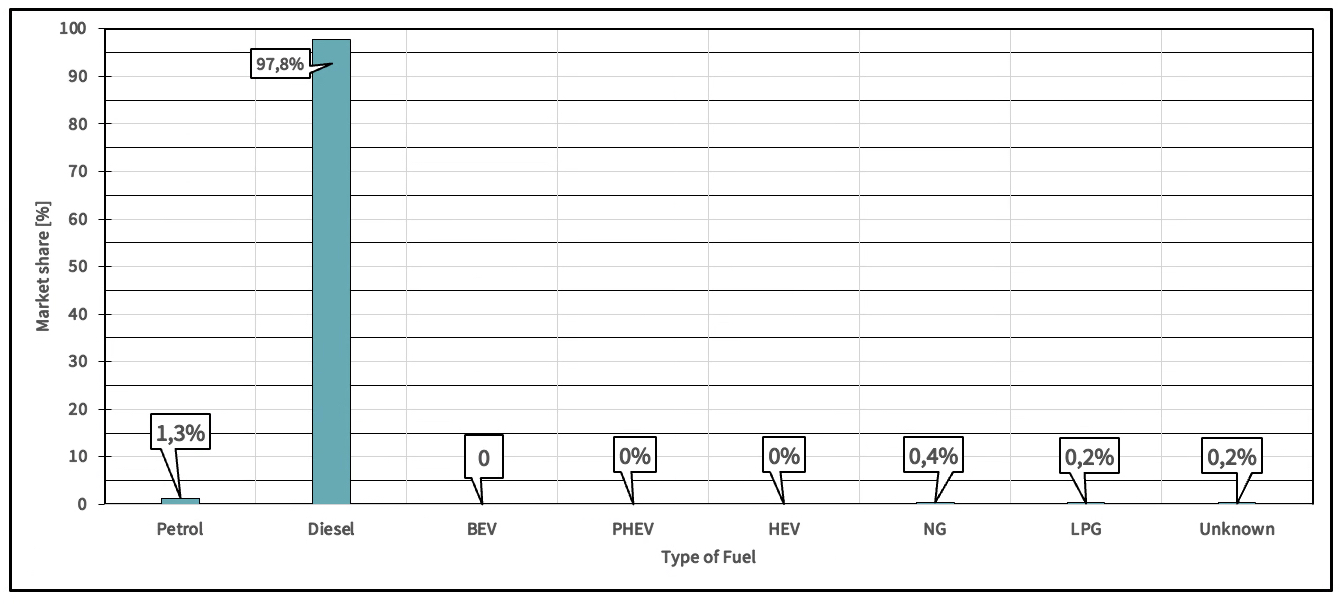
\includegraphics[width=0.7\textwidth]{Chapters/Pictures/Fuels_MarketShare.jpeg}
    \caption{Market share (in percentage) for different types of fuel}
    \label{fig:hdpower}
\end{figure}

So, in compliance with the sustainability goals given by the United Nations, it is necessary to renew also the Heavy Duty sector. In Table \ref{tab:dieselalternative} are shown the main options that can help us reach this objective:

\begin{table}[ht]
\centering
\begin{tabular}{|c|c|c|}
\hline
\rowcolor{bluepoli!40} \multicolumn{1}{|c|}{\textbf{Fuel}} & \multicolumn{1}{c|}{\textbf{PROS}}         & \multicolumn{1}{c|}{\textbf{CONS}} \\ \hline
\textbf{Biofuels} & Derivable from waste products & Still emit $CO_2$ during use \\ \hline
\textbf{Electricity} & \begin{tabular}[c]{@{}c@{}}$100\%$ clean during use; \\ Possible to couple the vehicle \\ with a fixed infrastructure \\ (OVH contact line)\end{tabular} & \begin{tabular}[c]{@{}c@{}}Cleanness depend on energetic mix; \\ Charging infrastructure and time \\ Weight of the battery\end{tabular} \\ \hline
\textbf{Hydrogen} & \begin{tabular}[c]{@{}c@{}}$100\%$ clean during use; \\ Higher energy density\end{tabular} & Lower volumetric density \\ \hline
\end{tabular}
\caption{Pros and Cons of different alternative fuels}
\label{tab:dieselalternative}
\end{table}

As said in a recent book\textsuperscript{\cite{Mazzo2021}}, the use of electric batteries in HD is not so convenient, because of their size and type of use, so we will focus on the $H_2$ technologies and how to produce this hydrogen in a sustainable way.

\section{Sate of the Art}
The field of production of hydrogen is in continuous development and actual technologies are the following\textsuperscript{\cite{guanda20211}}:
\begin{description}
    \item[Oil:] hydrogen is produced with steam reforming or partial oxidation from fossil or renewable oils;
    \item[Gas:] natural or bio-gas are hydrogen sources with steam reforming or partial oxidation;
    \item[Algae:] methods for utilising the photo-synthesis for hydrogen production;
    \item[Wood:] pyrolysis technology for hydrogen from biomass;
    \item[Power:] water electrolysis from renewable sources;
    \item[Coal:] with gasification technology hydrogen may be produced from coal;
    \item[Alcohols:] like hydrogen and methanol derived from gas or biomass (rich in hydrogen and may be reformed to hydrogen).
\end{description}

Due to the physical and geographical characteristics of Italy, we choose to feed the water electrolysis with the power generated by hydropower plant or by photovoltaic plant. This also needed to address the problem of being dependent from the foreign state, such in the case of oil and gas (and to their price fluctuation), that is a theme that started to spread in the last years.

\subsection{Electrolysis}
With electrolysis water is split in hydrogen and oxygen, in an electrochemical cell.

We can made a distinction about the solution based on the cell's temperature\textsuperscript{\cite{guanda20211}}.
\begin{itemize}
    \item Low temperature cells that can be divided into:
    \begin{description}
        \item[Alkaline electrolysis](Figure \ref{fig:alkaline})  based on a liquid solution of $NaOH$ or $KOH$;
        \item[PEM] (Figure \ref{fig:pem}) based on a polymeric electrolyte.
    \end{description}
    \item High temperature cells (such as SOEC).
\end{itemize}

Low temperature cells are already a commercial solution, while high temperature ones are still in development, so we will focus on the first one.

\begin{figure}[hp]
    \centering
    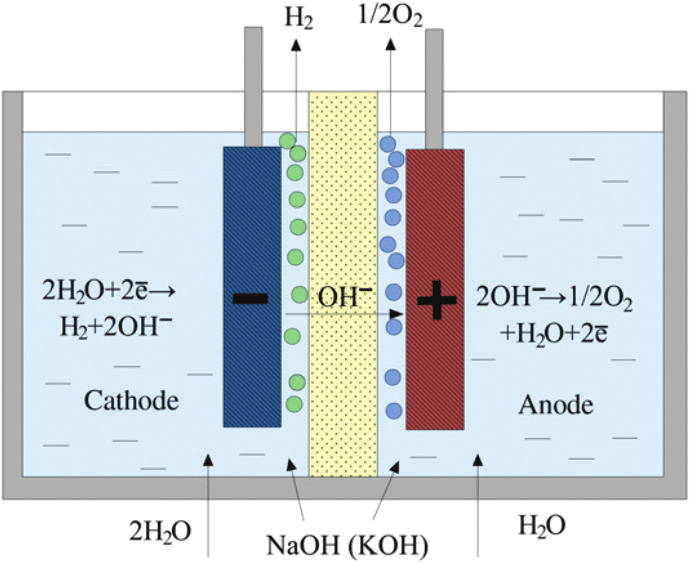
\includegraphics[width=0.5\textwidth]{Chapters/Pictures/Schematic-diagram-of-the-alkaline-electrolysis-cell-34.png}
    \caption{Schematic diagram of the alkaline electrolysis cell.
    (Courtesy of \textbf{\href{https://www.researchgate.net/figure/Schematic-diagram-of-the-alkaline-electrolysis-cell-34_fig4_327179309}{Scientific Figure on ResearchGate}})}
    \label{fig:alkaline}
\end{figure}

\begin{figure}[hp]
    \centering
    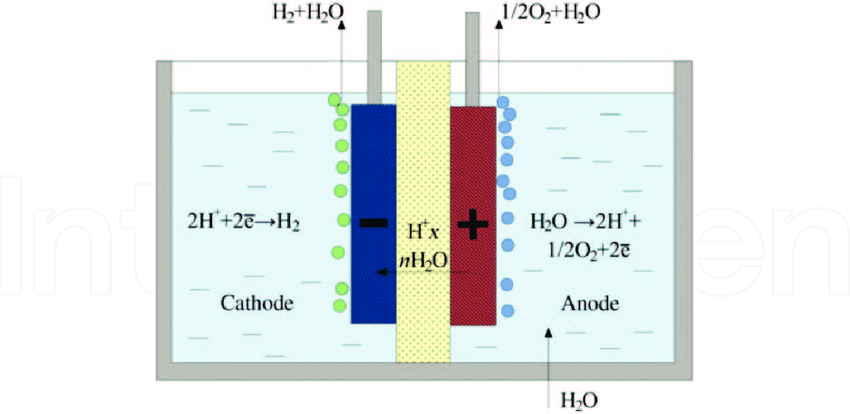
\includegraphics[width=0.8\textwidth]{Chapters/Pictures/Schematic-diagram-of-PEM-electrolysis-cell-33.png}
    \caption{Schematic diagram of PEM electrolysis cell.
    (Courtesy of \textbf{\href{https://www.researchgate.net/figure/Schematic-diagram-of-PEM-electrolysis-cell-33_fig1_327179309}{Scientific Figure on ResearchGate}})}
    \label{fig:pem}
\end{figure}

\subsection{Hydropower}
Hydropower plants use the potential energy of water flowing down to the turbine to produce electrical energy. We can find two main configurations\textsuperscript{\cite{lakohydro2010}}:
\begin{itemize}
    \item dams with reservoirs (Figure \ref{fig:dam}), that can be classified into:
    \begin{itemize}
        \item small dams;
        \item large dams;
        \item pumped storage;
    \end{itemize}
    \item run-of-the-river.
\end{itemize}

This technology does not produce significant $CO_2$ emissions other than those emitted during plants construction. 

It is also a mature technology: many of the plants that were built in the early decades of the $20^{th}$ century are currently still in operation. This reduces the costs of the facilities, because they consist simply in O$\&$M.

\begin{figure}[h]
    \centering
    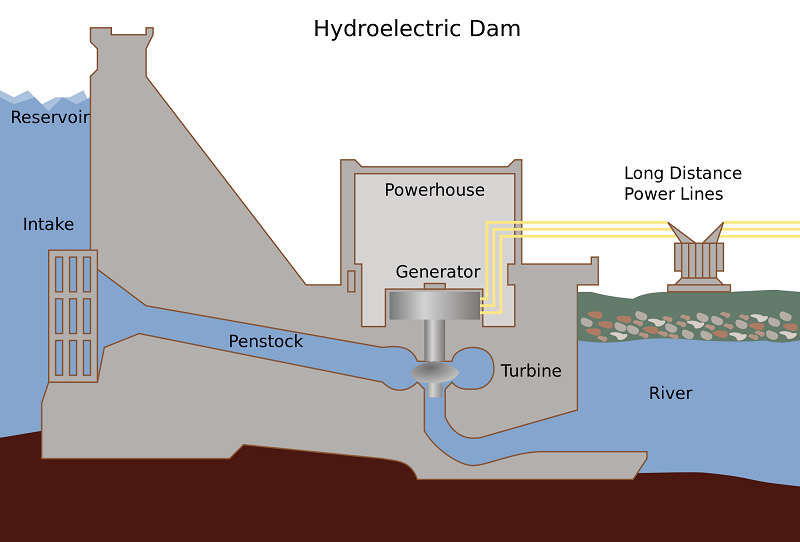
\includegraphics[width=0.6\textwidth]{Chapters/Pictures/Damparts.png}
    \caption{\small{A diagram showing the main components of a conventional hydroelectric facility.
    (Courtesy of \textbf{\href{https://energyeducation.ca/wiki/images/8/8e/Damparts.png}{energy education}})}}
    \label{fig:dam}
\end{figure}

Otherwise hydropower depends on rainfall and a reserve may be needed to compensate for periods of low rainfall. So, it will be possible that climate change influences the efficiency of such technology. We also have to take in account the political, societal and economic risk usual of this type of infrastructures.

\subsection{Photovoltaic}

\Huge{TO DO}